

%advantages
A major advantage of anonymous usage data is the fact that it captures developers in their natural habitat, without any observational bias. Deriving conclusions from hours of developers' field work is naturally more convincing than from hour-long, in-lab user studies. One of the types of questions that usage data is well-suited to answer are answerably by measuring the magnitude of an event. For instance, researchers might want to know ``How often do developers invoke the pull-up refactoring'' or ``How often is the file search invoked?''. By performing a count of a specific message in the collected logs researchers can easily calculate frequencies of specific actions, which can be often sufficient to answer important research questions. 

%disadvantages
However, researchers must be wary of a few common issues with magnitude analysis. First, in any sufficiently large set of user logs there is a small set of users that will use the feature/tool under analysis orders of magnitude more often than the general population, potentially skewing the data. Secondly, any fine-grained attempt to qualify the raw counts requires making possibly incorrect assumptions about the data. For instance, there is a temptation to report searchers per hour, yet any fine-grained time calculation requires assumptions about how time was spent between activities, which experience has taught us are often wrong. Note that coarse-grained qualification, such as searches performed per day, are possible.   

%example

\begin{figure}
  \centering
  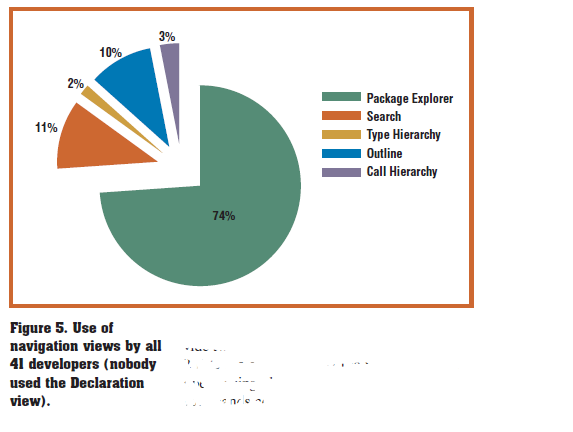
\includegraphics{AnalyzingUsageData/eclipse}
  \caption{Breakdown of Navigation-Focused View Usage in Eclipse}\label{fig:eclipse}
\end{figure}

One example of a study that reported exclusively magnitude data focused on which views and which commands do developers use within the Eclipse IDE... (How Are Java Software Developers Using the Eclipse IDE?)